\documentclass[withoutpreface,bwprint]{cumcmthesis}

\usepackage{float}
\usepackage{url}
\usepackage{booktabs}  
\usepackage{threeparttable} 
\usepackage{parskip}
\usepackage{subfigure}
\usepackage{epstopdf}
\usepackage{indentfirst}
\usepackage{graphics}
\setlength{\parindent}{1.5em}

\begin{document}
\section{实验目的}
实现一个PCA模型,能够对给定数据进行降维(即找到其中的主成分)


\section{实验要求}
\begin{enumerate}
\item 首先人工生成一些数据(如三维数据),让它们主要分布在低维空间中,如首先让某个维度的方差远小于其它唯独,然后对这些数据旋转。生成这些数据后,用你的PCA方法进行主成分提取。
\item 找一个人脸数据(小点样本量),用你实现PCA方法对该数据降维,找出一些主成分,然后用这些主成分对每一副人脸图像进行重建,比较一些它们与原图像有多大差别(用信噪比衡量)。
\end{enumerate}

\section{实验环境}
\begin{itemize}
\setlength{\itemindent}{1.5em}
\item 硬件:Intel i5-8265U、512G SSD、8G RAM;
\item 系统:Windows 11;
\item IDE:Pycharm。
\end{itemize}

\section{设计思想}
\subsection{算法原理}
有一个样本$\boldsymbol{x_{i}}$,其维度为$m$,其在基向量$\boldsymbol{u_{1}}$上的投影为
\begin{equation*}
z_{i1}=\boldsymbol{x_{i}'}\boldsymbol{u_{1}},
\end{equation*}

并且有
\begin{equation*}
\boldsymbol{u_{1}'}\boldsymbol{u_{1}}=1,
\end{equation*}

将之拓展到$m$个标准正交基向量$\boldsymbol{u_{1}}$、$\boldsymbol{u_{2}}\cdots\boldsymbol{u_{m}}$,则有
\begin{equation*}
z_{ij}=\boldsymbol{x_{i}'}\boldsymbol{u_{j}},j=1,2\cdots m
\end{equation*}
\begin{equation*}
\boldsymbol{z_{i}'}=\begin{bmatrix}z_{i1}&z_{i2}&\cdots&z_{im}\end{bmatrix},
\end{equation*}

$\boldsymbol{z_{i}}$可以视为$\boldsymbol{x_{i}}$在基向量$\boldsymbol{u_{1}}$、$\boldsymbol{u_{2}}\cdots\boldsymbol{u_{m}}$构成的向量空间上的投影。

不妨设
\begin{equation*}
\boldsymbol{y_{i}}=\sum_{j=i}^{m}z_{ij}\boldsymbol{u_{j}}=\sum_{j=i}^{m}(\boldsymbol{x_{i}'u_{j}})\boldsymbol{u_{j}},
\end{equation*}

我们可以将$\boldsymbol{z_{i}}$视为$\boldsymbol{x_{i}}$的压缩后的向量,$\boldsymbol{y_{i}}$视为解压后的向量,$\left \|\boldsymbol{x_{i}}-\boldsymbol{y_{i}}\right \|^{2}$视为样本压缩后的损失。

显然当基向量数目为$m$时,压缩损失为0,但此时并未起到压缩效果。要起到压缩效果,需要让$\boldsymbol{z_{i}}$维度降低,即减少基向量的数目。不妨设基向量的数目减少到$k$,那么此时压缩后的样本$\boldsymbol{z_{i}}$,还原后的样本$\boldsymbol{y_{i}}$,压缩导致的误差$\boldsymbol{\Delta_{i}}$为:
\begin{equation}
\boldsymbol{z_{i}'}=\begin{bmatrix}z_{i1}&z_{i2}&\cdots&z_{ik}\end{bmatrix}=\begin{bmatrix}\boldsymbol{x_{i}'u_{1}}&\boldsymbol{x_{i}'u_{2}}&\cdots&\boldsymbol{x_{i}'u_{k}}\end{bmatrix},
\end{equation}
\begin{equation}
\boldsymbol{y_{i}}=\sum_{j=i}^{k}z_{ij}\boldsymbol{u_{j}}=\sum_{j=i}^{k}(\boldsymbol{x_{i}'u_{j}})\boldsymbol{u_{j}},
\end{equation}
\begin{equation}
\boldsymbol{\Delta_{i}}=\sum_{j=k+1}^{m}z_{ij}\boldsymbol{u_{j}}=\sum_{j=k+1}^{m}(\boldsymbol{x_{i}'u_{j}})\boldsymbol{u_{j}},
\end{equation}

现在给定压缩的维度$k$,要求的一组基向量,使压缩的总体误差尽可能小。不妨设数据集为$\boldsymbol{X}$,样本数量为$n$,每一个样本维度为$m$,总误差为$S$。

\begin{equation*}
S=\sum_{i=1}^{n}\left \| \boldsymbol{\Delta_{i}} \right \|^{2}=\sum_{i=1}^{n}\sum_{j=k+1}^{m}(\boldsymbol{x_{i}'u_{j}})\boldsymbol{u_{j}},
\end{equation*}

为后续推导的方便,将基向量组织为
\begin{equation*}
\boldsymbol{U_{k}}=\begin{bmatrix}\boldsymbol{u_{1}}&\boldsymbol{u_{2}}&\cdots&\boldsymbol{u_{k}}\end{bmatrix},
\end{equation*}
\begin{equation*}
\boldsymbol{U_{m-k}}=\begin{bmatrix}\boldsymbol{u_{k+1}}&\boldsymbol{u_{k+2}}&\cdots&\boldsymbol{u_{m}}\end{bmatrix}.
\end{equation*}

将式(1)、式(2)、式(3)改写为向量内积、矩阵乘法的形式,
\begin{equation}
\boldsymbol{z_{i}}=\boldsymbol{U_{k}'x_{i}},
\end{equation}
\begin{equation}
\boldsymbol{y_{i}}=\sum_{j=i}^{k}z_{ij}\boldsymbol{u_{j}}=\boldsymbol{U_{k}z_{i}}=\boldsymbol{U_{k}U_{k}'x_{i}},
\end{equation}
\begin{equation}
\boldsymbol{\Delta_{i}}=\sum_{j=k+1}^{m}z_{ij}\boldsymbol{u_{j}}=\boldsymbol{U_{m-k}U_{m-k}'x_{i}}.
\end{equation}

不妨设数据集$\boldsymbol{X}$为
\begin{equation*}
\boldsymbol{X}=\begin{bmatrix}\boldsymbol{x_{1}}&\boldsymbol{x_{2}}&\cdots&\boldsymbol{x_{n}}\end{bmatrix}.
\end{equation*}

则式(4)、式(5)、式(6)可以进一步写作:
\begin{equation*}
\boldsymbol{Z}=\boldsymbol{U_{k}X},
\end{equation*}
\begin{equation*}
\boldsymbol{Y}=\boldsymbol{U_{k}U_{k}'X},
\end{equation*}
\begin{equation*}
\boldsymbol{\Delta}=\boldsymbol{U_{m-k}U_{m-k}'X},
\end{equation*}

上式$\boldsymbol{\Delta}$中每一列为一个样本的误差,所求$\boldsymbol{U}$即为使总误差$S$最小的向量。
\begin{equation*}
\begin{aligned}
S&=tr(\boldsymbol{\Delta'\Delta})\\
&=tr(\boldsymbol{X'U_{m-k}U_{m-k}'U_{m-k}U_{m-k}'X})\\
&=tr(\boldsymbol{X'U_{m-k}U_{m-k}'X})\\
&=tr(\boldsymbol{U_{m-k}'XX'U_{m-k}})\\
\end{aligned}
\end{equation*}

不妨设此时$X$是去中心化之后的数据集,则有
\begin{equation*}
\boldsymbol{D}=\boldsymbol{XX'},
\end{equation*}
\begin{equation}
S=tr(\boldsymbol{U_{m-k}'DU_{m-k}}),
\end{equation}

式中$\boldsymbol{D}$为数据集$\boldsymbol{X}$的协方差矩阵,是一个$m\times m$的实对称阵,其有$m$个特征值与特征向量。不妨设其某一个特征向量为$\boldsymbol{p_{1}}$,对应的特征值为$\lambda_{1}$,则有
\begin{equation*}
\boldsymbol{Dp_{1}}=\lambda_{1}\boldsymbol{p_{1}},
\end{equation*}
\begin{equation*}
\begin{aligned}
\boldsymbol{D}\begin{bmatrix}\boldsymbol{p_{1}}&\boldsymbol{p_{2}}&\cdots&\boldsymbol{p_{m-k}}\end{bmatrix}
&=\begin{bmatrix}\lambda_{1}\boldsymbol{p_{1}}&\lambda_{2}\boldsymbol{p_{2}}&\cdots&\lambda_{m-k}\boldsymbol{p_{m-k}}\end{bmatrix}\\
&=\begin{bmatrix}\boldsymbol{p_{1}}&\boldsymbol{p_{2}}&\cdots&\boldsymbol{p_{m-k}}\end{bmatrix}\begin{bmatrix}\lambda_{1}& & & \\ &\lambda_{2}& & \\ & &\ddots& \\ & & &\lambda_{m-k}\\\end{bmatrix}\\
&=\boldsymbol{P_{m-k}\Lambda_{m-k}}\\
\end{aligned}
\end{equation*}

由于实对称阵的特征向量是正交标准化的,故
\begin{equation*}
\boldsymbol{P_{m-k}'P_{m-k}}=\boldsymbol{E_{(m-k)\times (m-k)}}
\end{equation*}
\begin{equation*}
\boldsymbol{DP_{m-k}}=\boldsymbol{P_{m-k}\Lambda_{m-k}}
\end{equation*}
\begin{equation}
\boldsymbol{P_{m-k}'DP_{m-k}}=\boldsymbol{\Lambda_{m-k}}
\end{equation}

综合来看式(7)、式(8)的形式,$\boldsymbol{U_{m-k}}$如果选取的是$\boldsymbol{D}$的特征向量,那么为了使$\boldsymbol{U_{m-k}'DU_{m-k}}$最小,应该选取$m-k$个最小的特征值对应的特征向量。但如果$\boldsymbol{U_{m-k}}$中某个基向量选取的不是$\boldsymbol{D}$的特征向量,则该基向量可以视作由几个特征向量构成,最后的迹仍可以看作为特征值的组合。$\boldsymbol{U_{m-k}}$选取了$m-k$个最小的特征值对应的特征向量,则$\boldsymbol{U_{k}}$选取的是其他$k$个特征向量。

最后推导得出基向量$U_{k}$为中心化后的$\boldsymbol{X}$的协方差矩阵的前$k$个特征值对应的特征向量。压缩后的数据为$\boldsymbol{U_{k}X}$。还原的数据为$\boldsymbol{U_{k}U_{k}'X}$。

\subsection{程序设计}
\subsubsection{数据生成}
使用numpy.random.multivariate\_normal函数生成一定数量的数据,为了压缩的效果,需要使某一个维度的方差相对较小,以使得压缩误差尽可能小。

\subsubsection{图片读取}
图片读取使用了cv2.read函数将图片转化为一个矩阵,使用了cv2.cvtcolor函数将矩阵变成灰度矩阵。

\subsubsection{PCA实现}
首先对输入的矩阵进行去中心化的操作,然后求得其协方差矩阵,然后调用numpy.linalg.eig函数得到其特征值、特征向量,取前$k$大的特征值对应的特征向量作为压缩的基向量,然后依据上述公式对原数据进行压缩,压缩后基于之前的基向量还原,并且加上中心值,即完成了解压缩。

\section{实验结果与分析}
\subsection{生成数据}
下图为二维、三维数据压缩一个维度的压缩效果。其中绿色点表示原始数据,红色点表示解压缩后的数据,图中的直线表示基向量。
\begin{figure}[H]
    \centering
    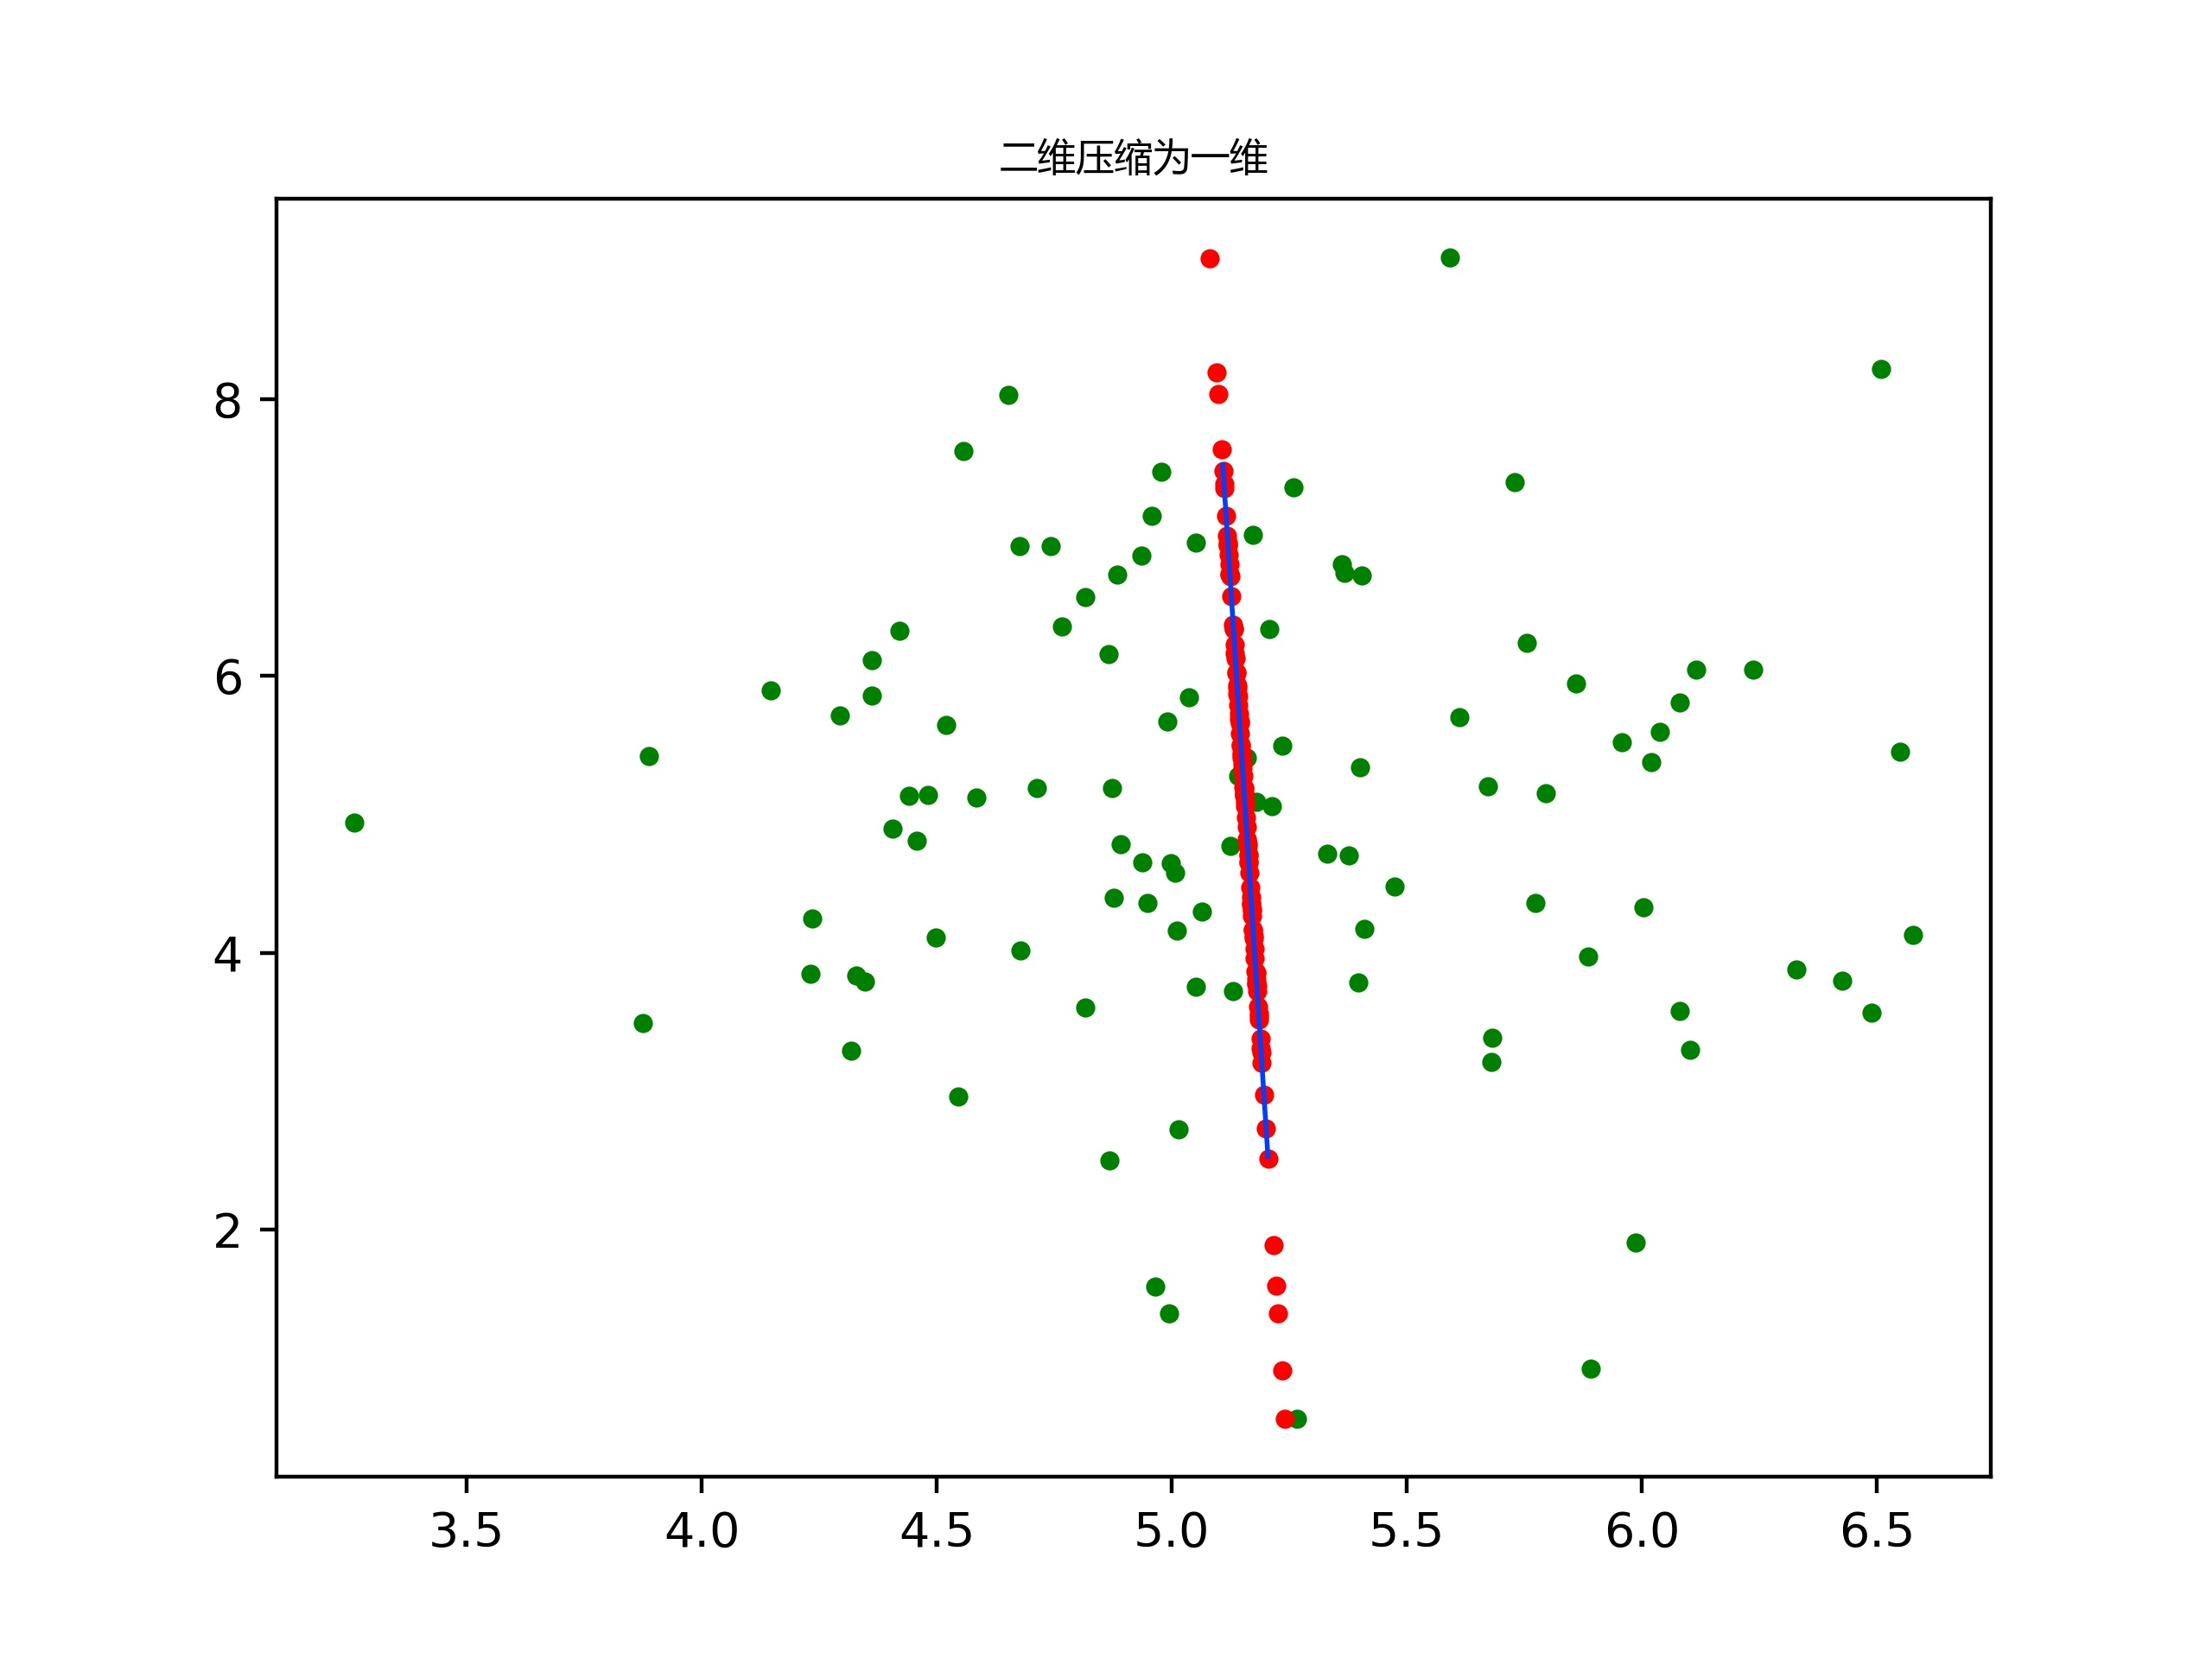
\includegraphics[width=\textwidth]{二维}
    \caption{二维压缩效果}
    \label{图1}
\end{figure}
该图是从垂直于压缩平面的方向观察,可以看到绿色点和红色点几乎重合,压缩可以看作绿色点投影到平面上成为了红色点。
\begin{figure}[H]
    \centering
    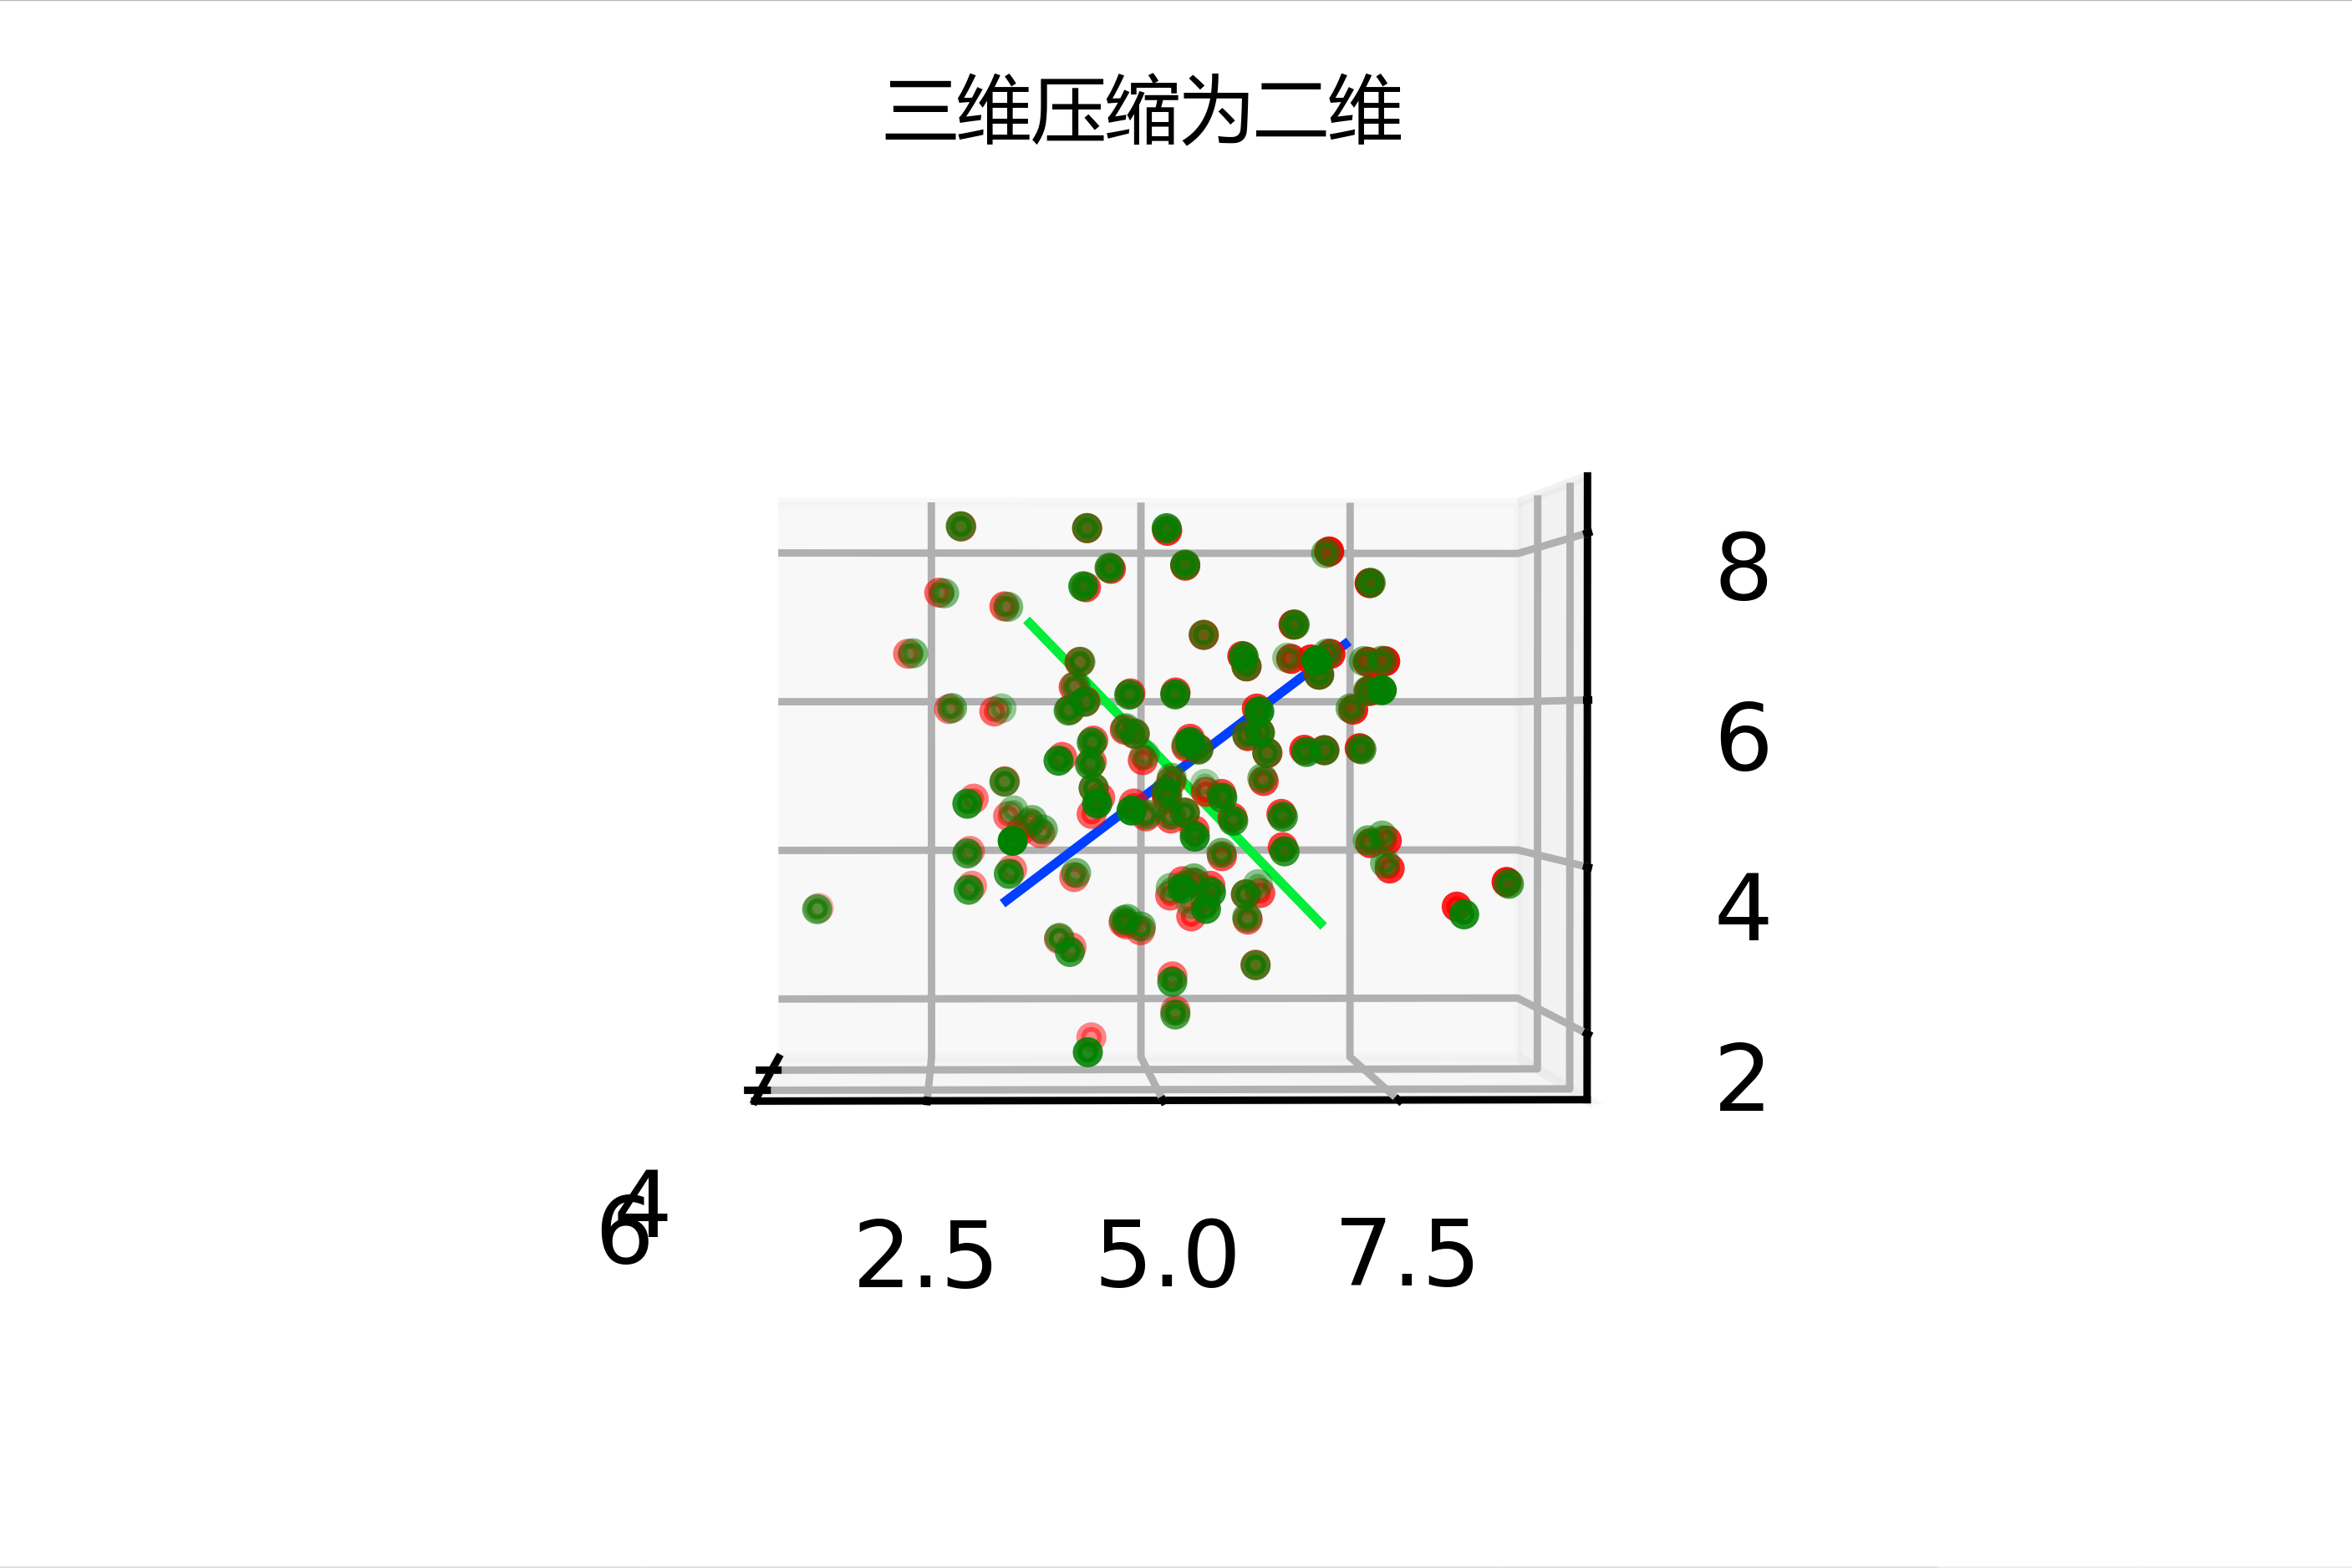
\includegraphics[width=0.7\textwidth]{三维一}
    \caption{三维压缩效果一}
    \label{图2}
\end{figure}
该图为平行于压缩平面的方向观察,可以看到红色点在此视角下成为了一条直线。
\begin{figure}[H]
    \centering
    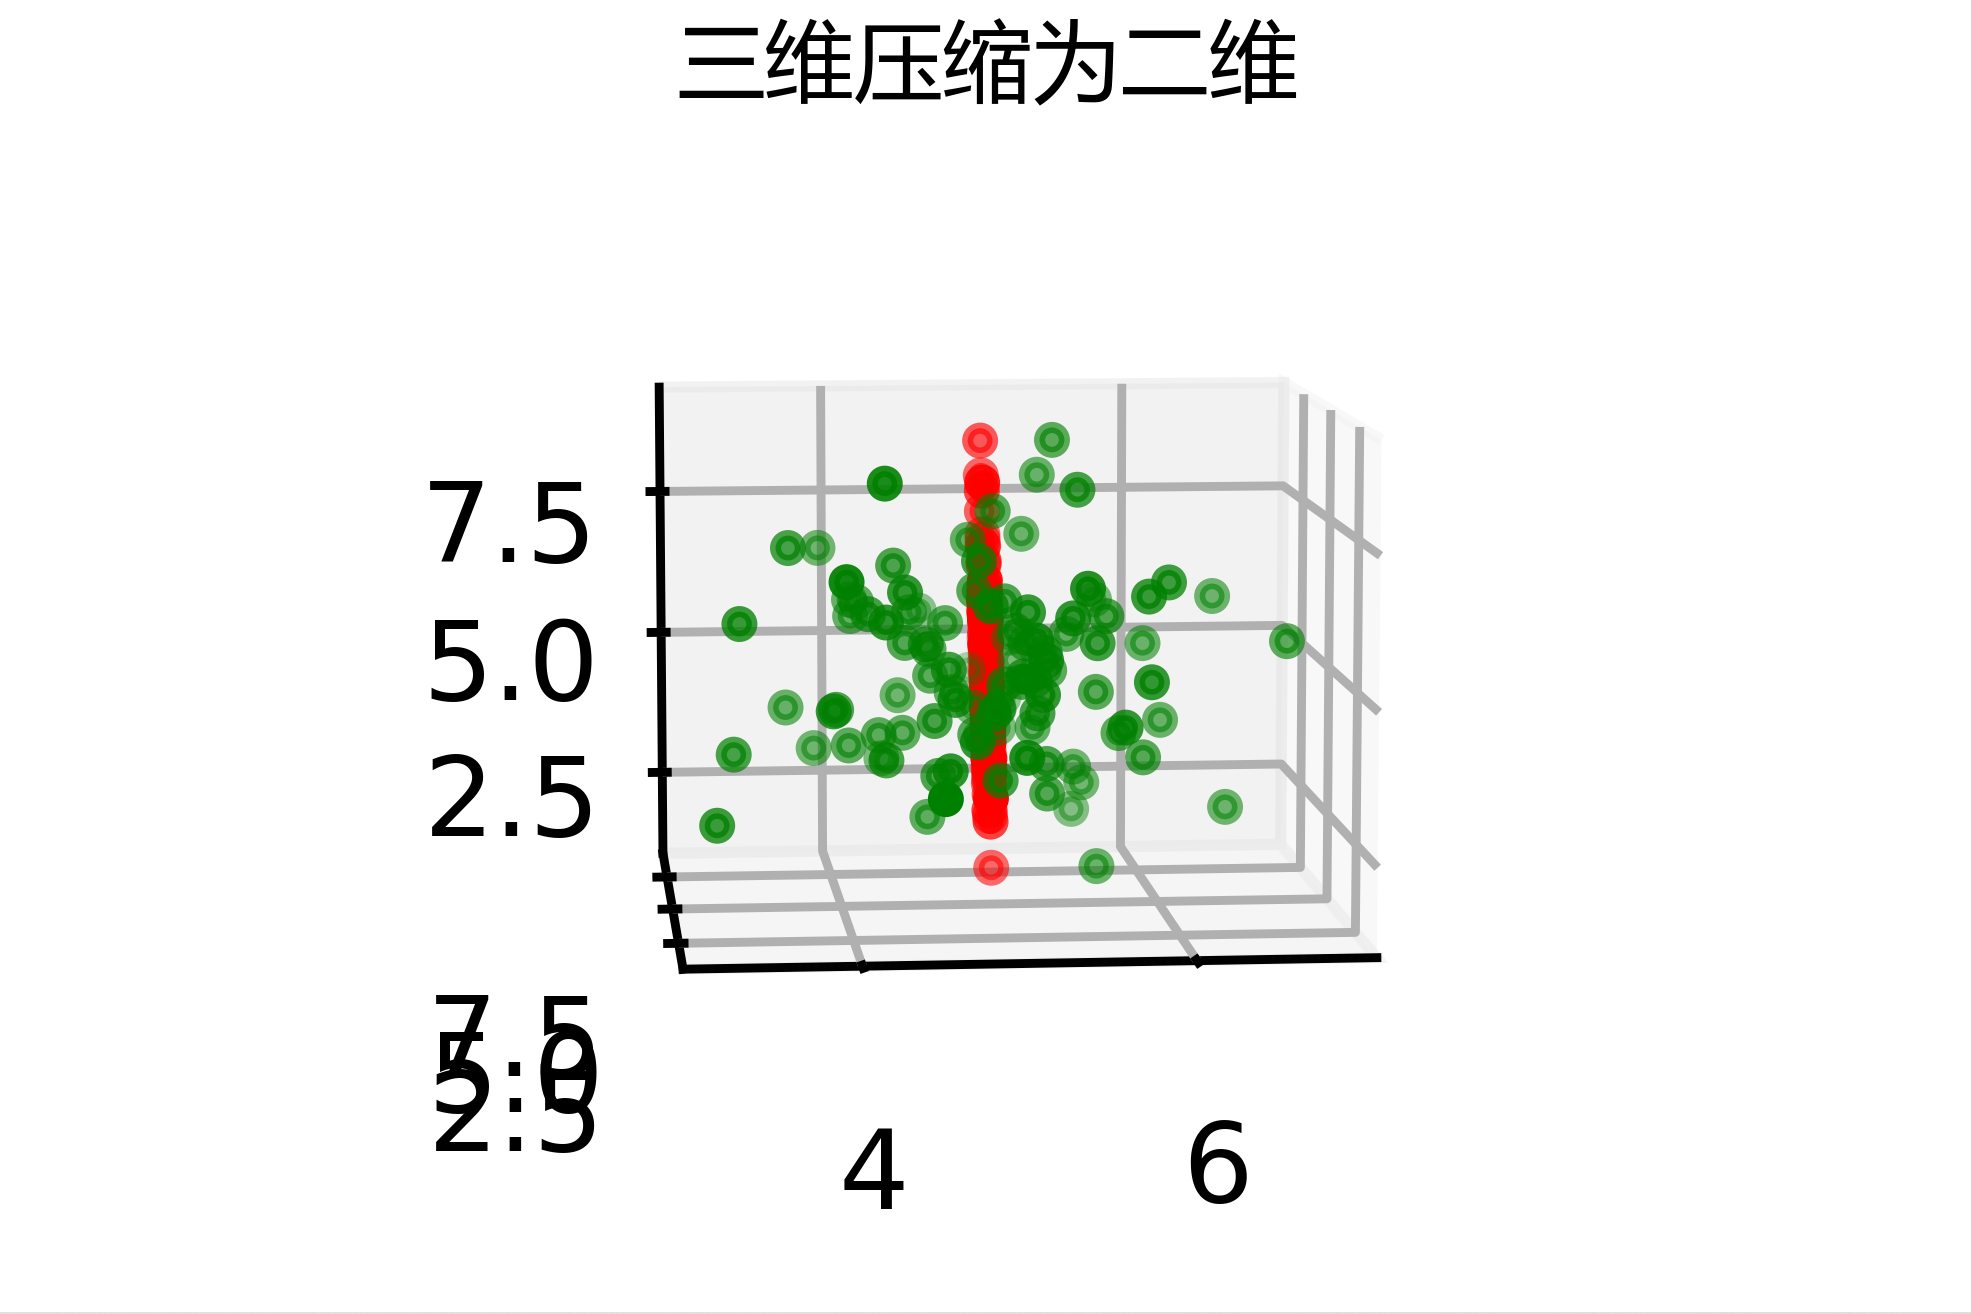
\includegraphics[width=0.7\textwidth]{三维二}
    \caption{三维压缩效果二}
    \label{图3}
\end{figure}
\subsection{图片数据}
本次实验选取了五幅图片,先将其转化为灰度图后,然后进行压缩。解压缩图片以及PSNR如图所示。
\begin{figure}[H]
    \centering
    
\includegraphics[width=\textwidth]{trump}
    \caption{图片压缩例一}
    \label{图4}
\end{figure}
\begin{figure}[H]
    \centering
    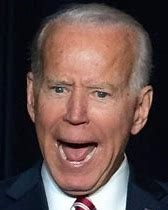
\includegraphics[width=\textwidth]{biden}
    \caption{图片压缩例二}
    \label{图5}
\end{figure}
\begin{figure}[H]
    \centering
    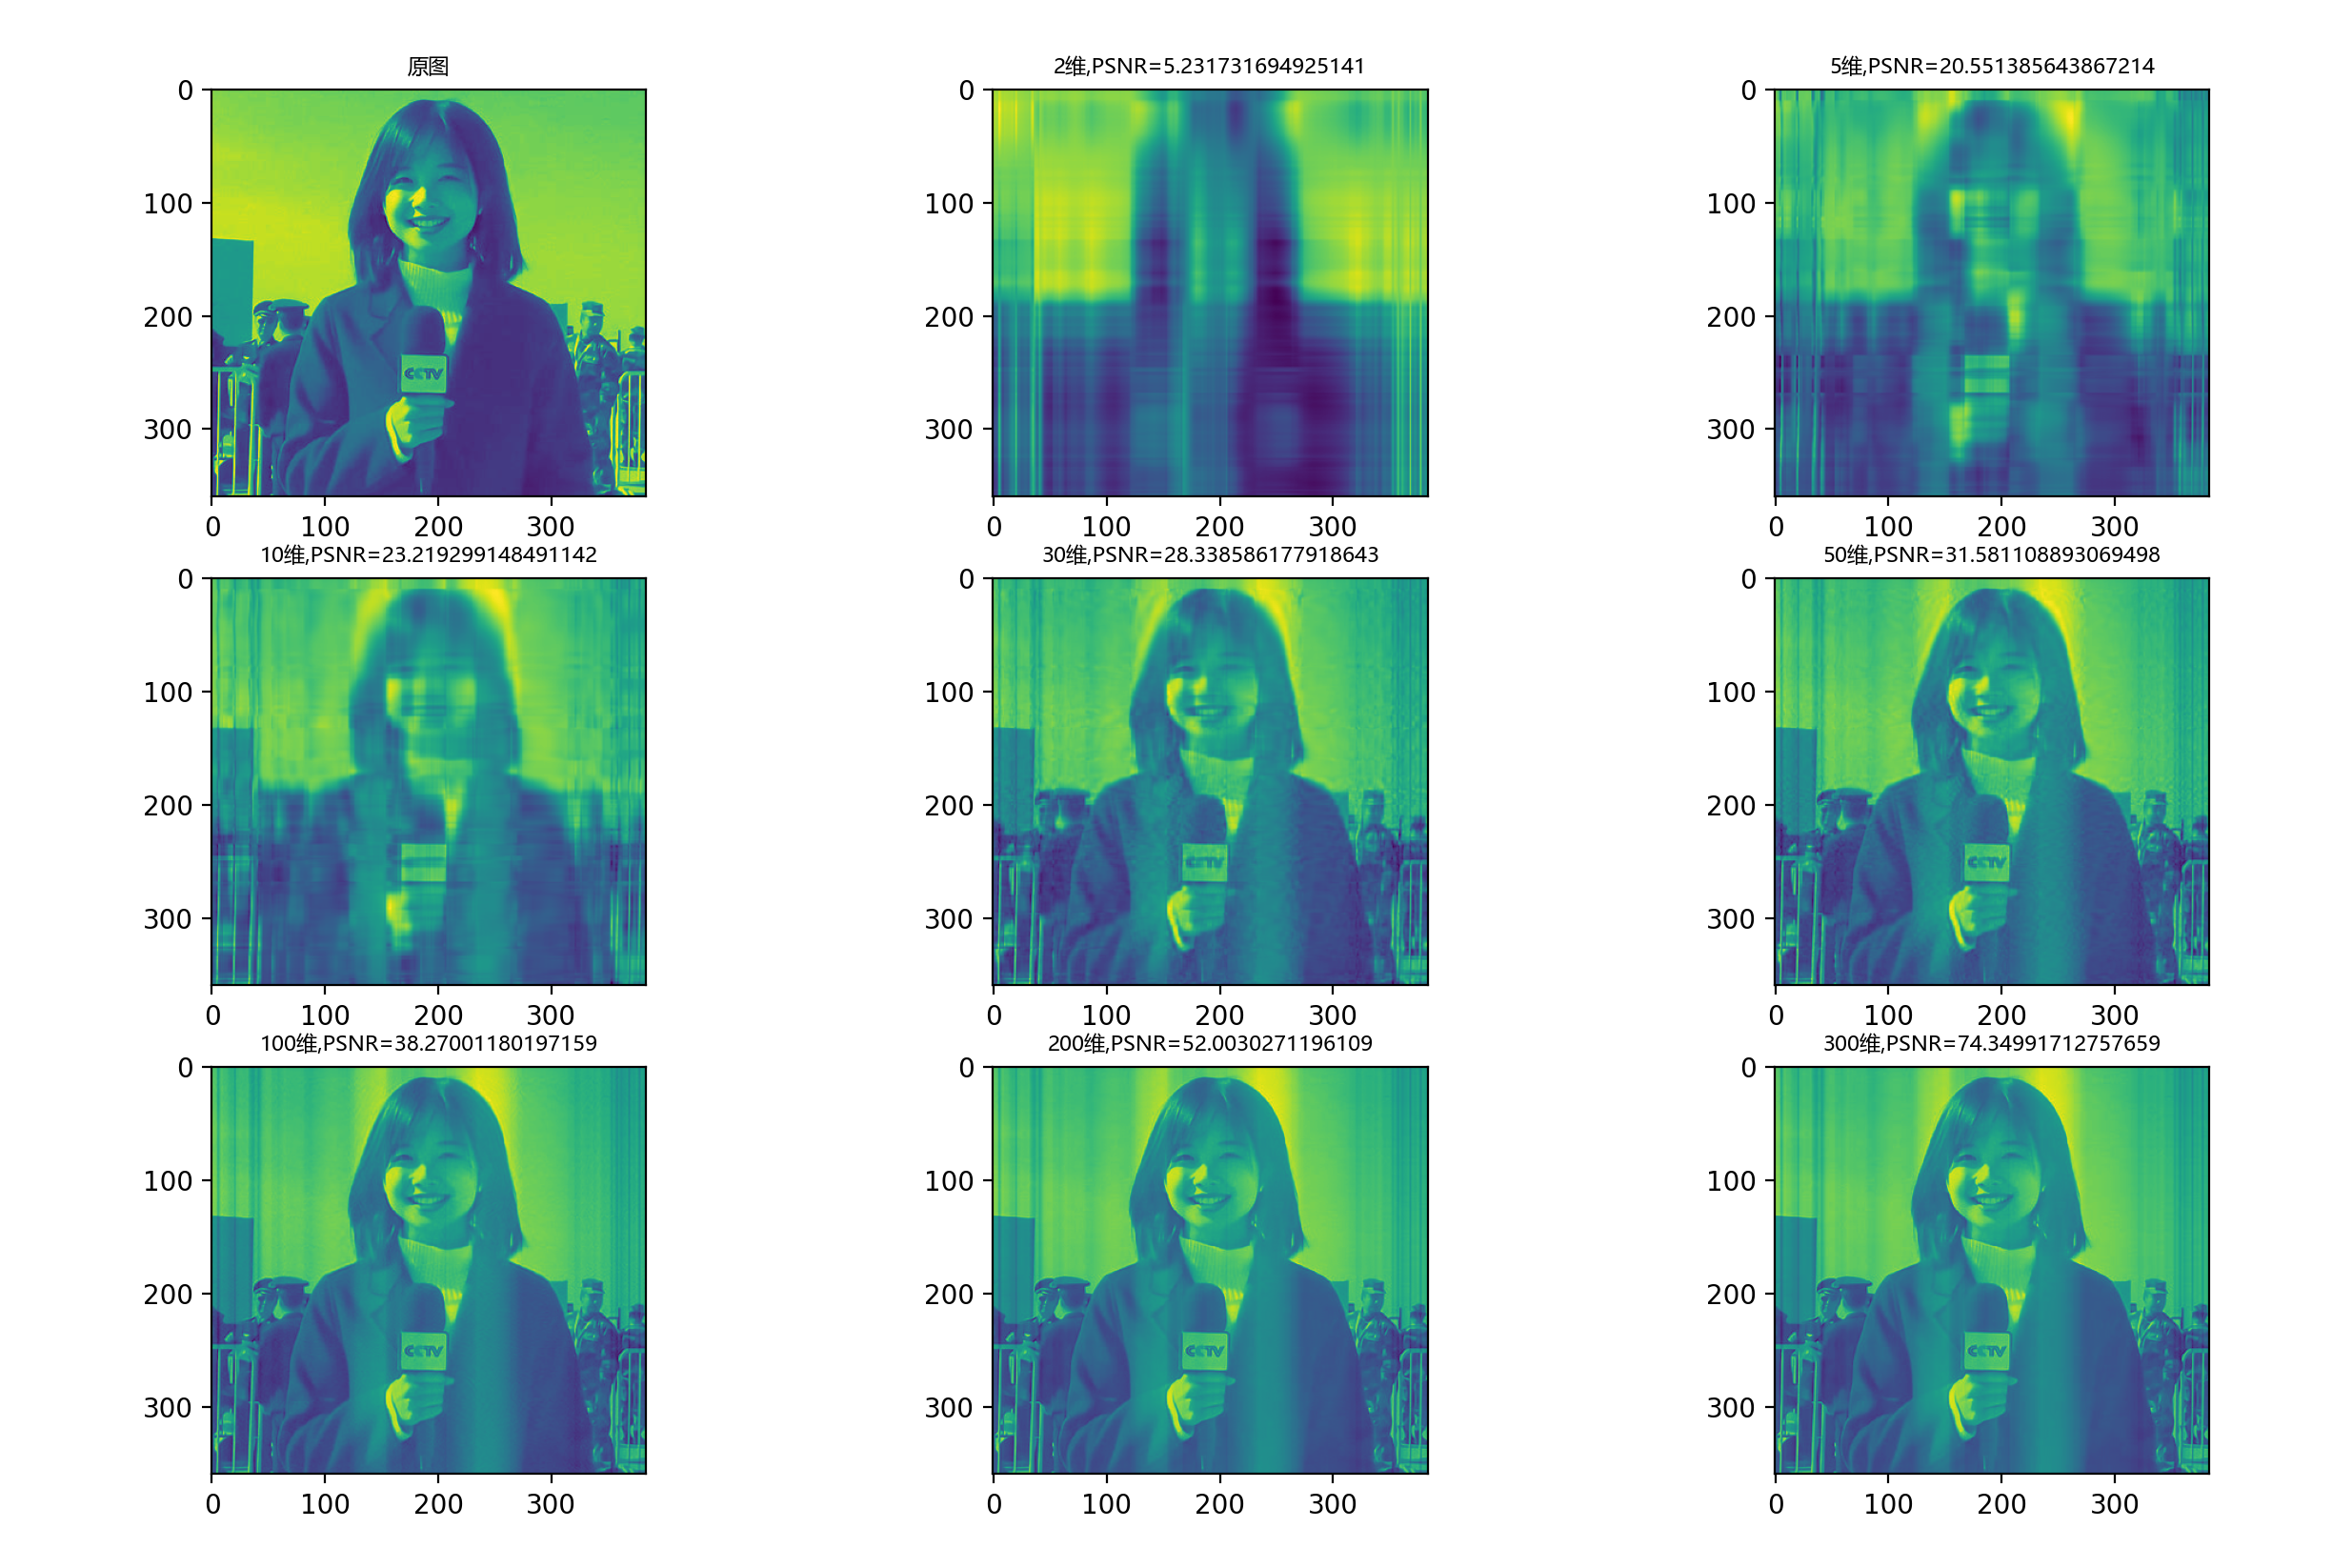
\includegraphics[width=\textwidth]{wbb1}
    \caption{图片压缩例三}
    \label{图6}
\end{figure}
\begin{figure}[H]
    \centering
    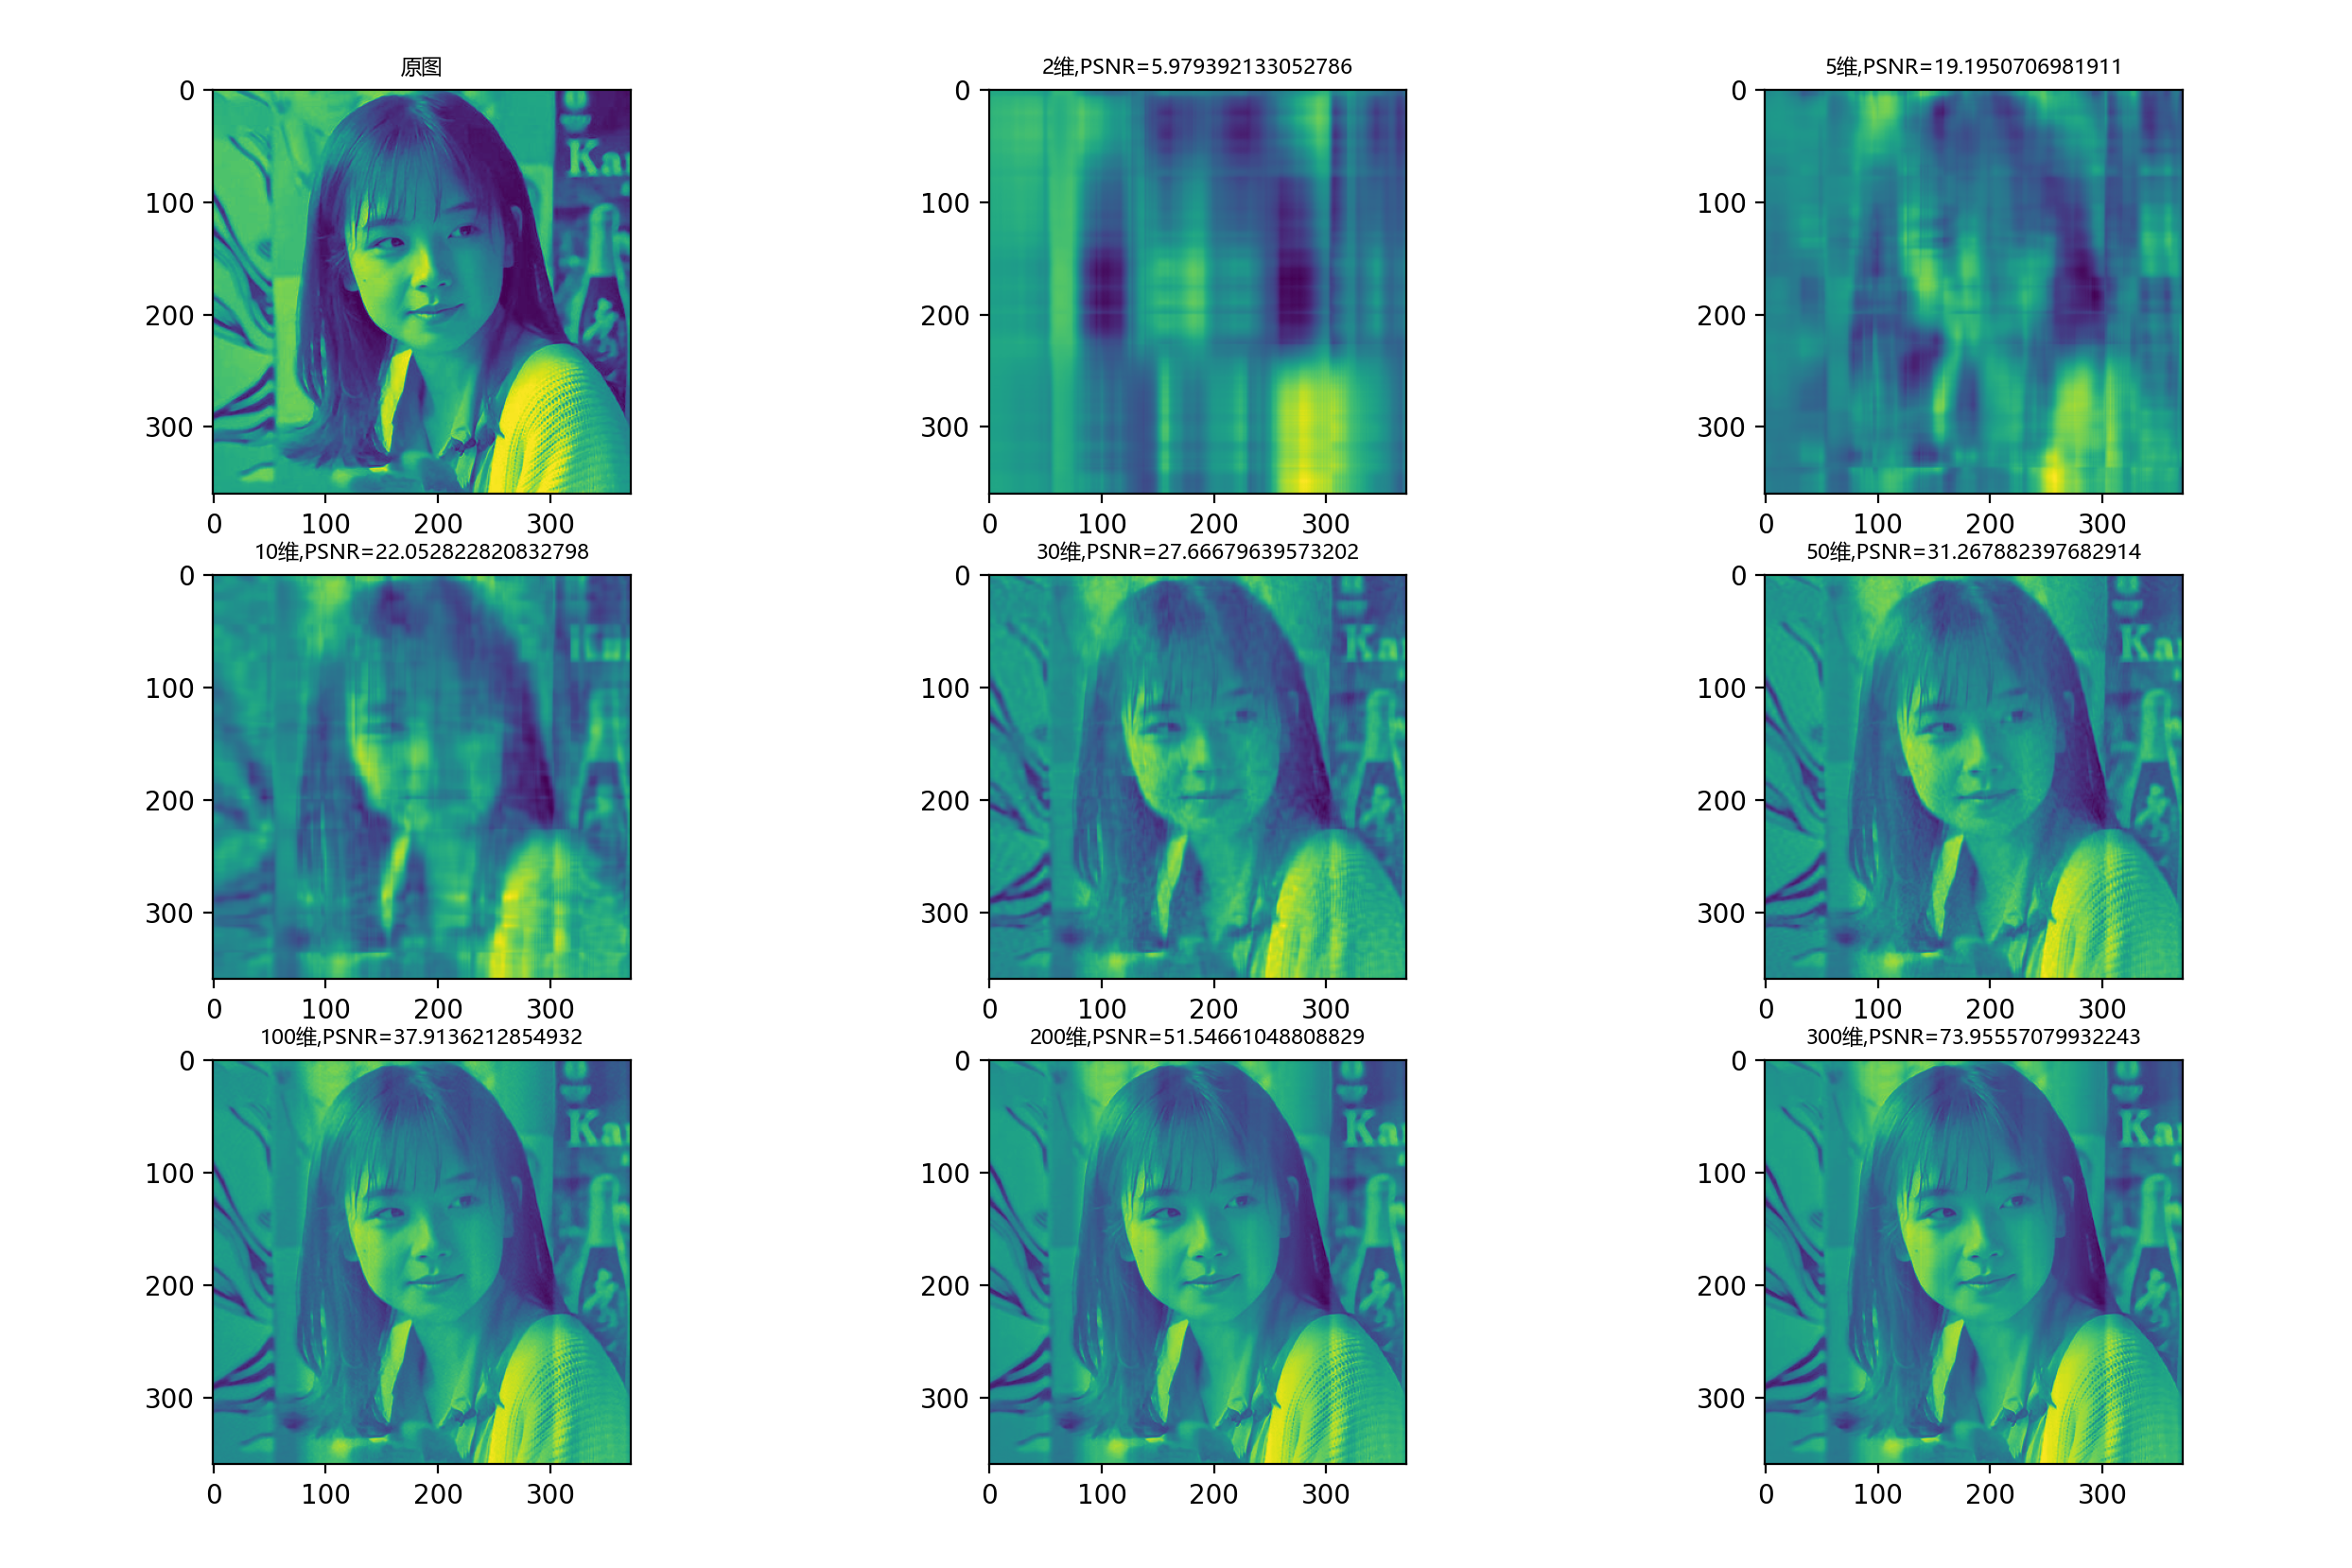
\includegraphics[width=\textwidth]{wbb2}
    \caption{图片压缩例四}
    \label{图7}
\end{figure}
\begin{figure}[H]
    \centering
    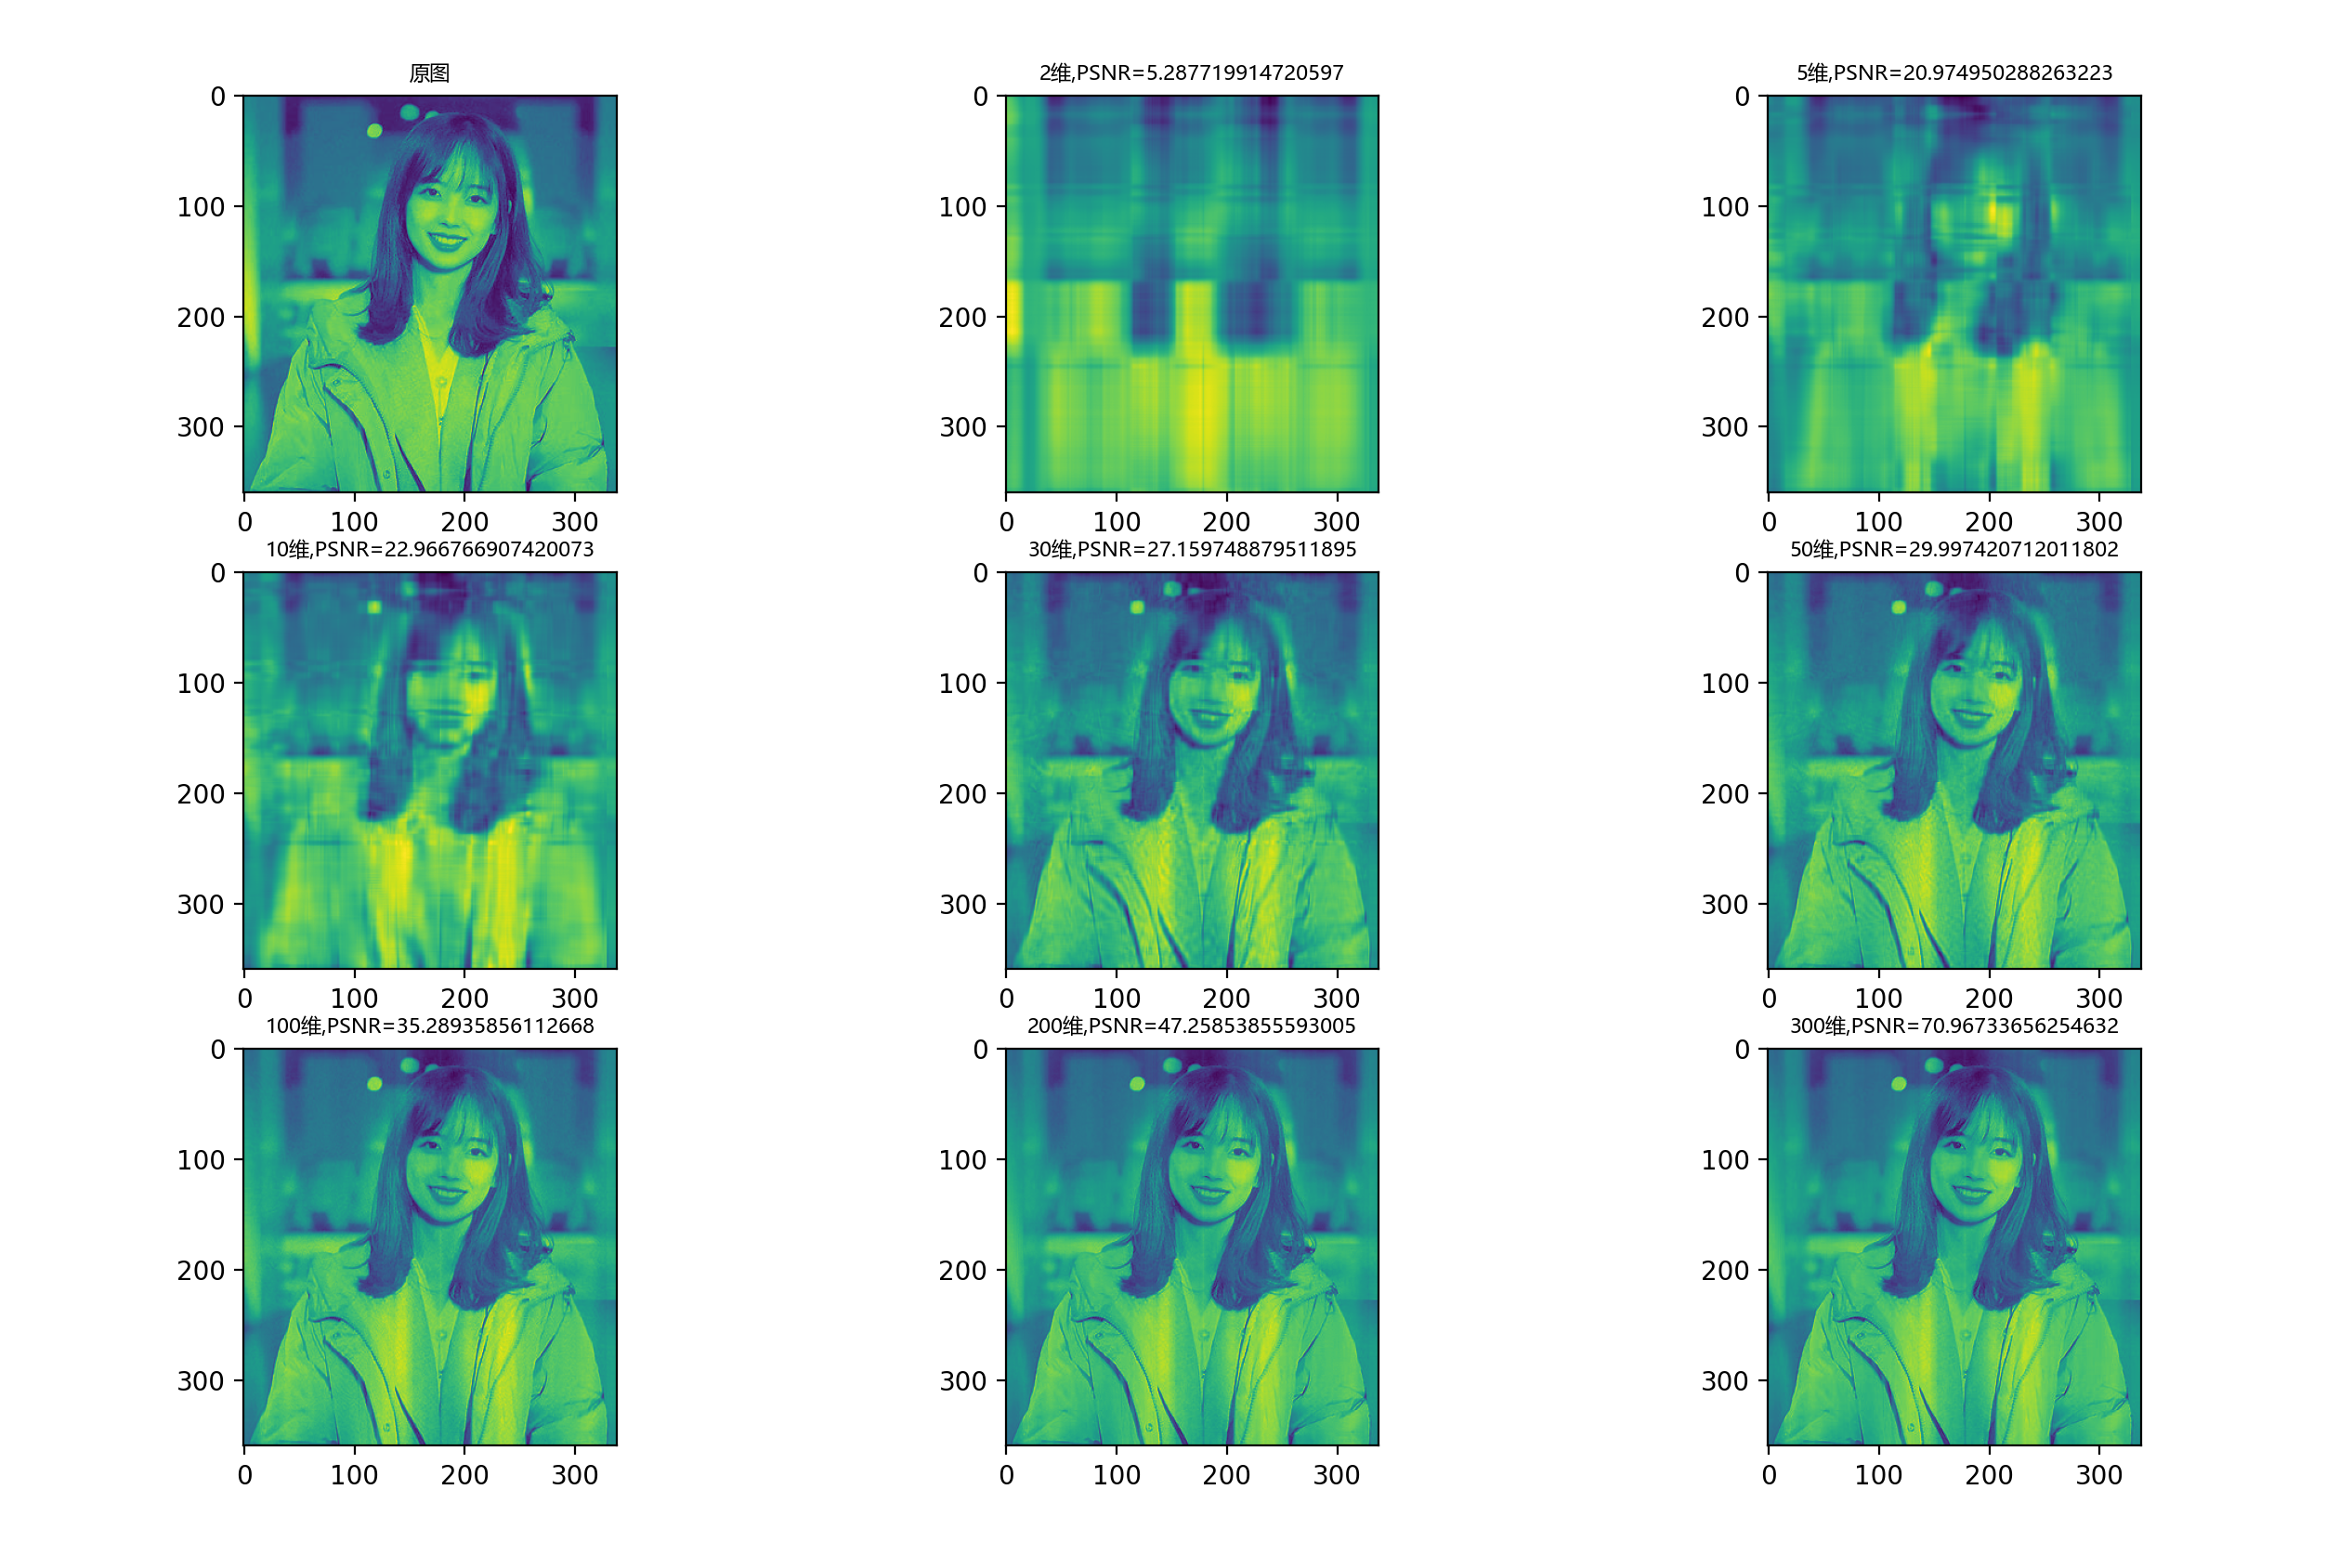
\includegraphics[width=\textwidth]{wbb3}
    \caption{图片压缩例五}
    \label{图8}
\end{figure}
\section{结论}
PCA通过舍弃某些维度上变化较小的信息,降低了数据的维度,有效的实现了数据的压缩存储。但PCA也有一定的缺陷,不同维度的数据其重要程度是不同的,不能简单的依据方差或是特征值来衡量,数据集不同维度的重要性并不没有保存在数据集中。

\newpage
\begin{appendix}
\section{主程序}
\begin{lstlisting}[language=python]
import copy

import numpy as np
import cv2

from graph import init_graph, font_title, draw_graph
import matplotlib.pyplot as plt


def generate_data(size, raw_dimension_num):
    mean_list = [5.0] * raw_dimension_num
    cov_list = [[0.0] * i + [2.0] + [0.0] * (raw_dimension_num - i - 1) for i in range(raw_dimension_num)]
    cov_list[0][0] = 0.5

    data = np.random.multivariate_normal(mean_list, cov_list, size)
    return data


def PCA(data, compress_dimension_num):
    raw_dimension_num = len(data[0])
    mean_array = np.mean(data, axis=0)
    for i in range(len(data)):
        data[i] -= mean_array

    cov_matrix = (data.T @ data) / len(data)
    eigenvalues, eigenvectors = np.linalg.eig(cov_matrix)
    sort_index = np.argsort(eigenvalues)
    # 鍙樻崲鐭╅樀 or 鏈�绉讳綅鐨勫熀鍚戦噺
    compress_matrix = np.array([[0.0] * compress_dimension_num] * raw_dimension_num)
    for i in range(compress_dimension_num):
        index = sort_index[-1 - i]
        compress_matrix[:, i] = eigenvectors[:, index]

    # 鍘嬬缉鍚庣殑鐭╅樀
    compressed_data = data @ compress_matrix

    # 瑙e帇鍚庣殑鐭╅樀
    decompressed_data = compressed_data @ compress_matrix.T
    for i in range(len(data)):
        # 鍔犱笂涓�蹇冨€�
        decompressed_data[i] += mean_array

    return mean_array, compress_matrix, compressed_data, decompressed_data


def draw(data, decompressed_data, mean_array, compress_matrix):
    raw_dimension_num = len(data[0])

    if raw_dimension_num == 2:
        init_graph(plt, dpi=400)
        plt.title("浜岀淮鍘嬬缉涓轰竴缁�", font=font_title)
        plt.scatter(data[:, 0], data[:, 1], c='g', marker='.')
        plt.scatter(decompressed_data[:, 0], decompressed_data[:, 1], c='r', marker='.')
        plt.plot([mean_array[0] - 2.5 * compress_matrix[0][0], mean_array[0] + 2.5 * compress_matrix[0][0]],
                 [mean_array[1] - 2.5 * compress_matrix[1][0], mean_array[1] + 2.5 * compress_matrix[1][0]], linewidth=1)
        draw_graph(plt)
    elif raw_dimension_num == 3:
        init_graph(plt, dpi=400)
        ax = plt.axes(projection='3d')
        plt.title("涓夌淮鍘嬬缉涓轰簩缁�", font=font_title)
        ax.scatter3D(data[:, 0], data[:, 1], data[:, 2], c='g', marker='.')
        ax.scatter3D(decompressed_data[:, 0], decompressed_data[:, 1], decompressed_data[:, 2], c='r', marker='.')
        ax.plot3D([mean_array[0] - 2.5 * compress_matrix[0][0], mean_array[0] + 2.5 * compress_matrix[0][0]],
                  [mean_array[1] - 2.5 * compress_matrix[1][0], mean_array[1] + 2.5 * compress_matrix[1][0]],
                  [mean_array[2] - 2.5 * compress_matrix[2][0], mean_array[2] + 2.5 * compress_matrix[2][0]], linewidth=1)
        ax.plot3D([mean_array[0] - 2.5 * compress_matrix[0][1], mean_array[0] + 2.5 * compress_matrix[0][1]],
                  [mean_array[1] - 2.5 * compress_matrix[1][1], mean_array[1] + 2.5 * compress_matrix[1][1]],
                  [mean_array[2] - 2.5 * compress_matrix[2][1], mean_array[2] + 2.5 * compress_matrix[2][1]], linewidth=1)
        draw_graph(plt)
    else:
        print("Matplotlib can't draw if dimension num>3")


def PSNR(img1, img2):
    img0 = img1 - img2
    return 10 * np.log10(65025 * len(img0) * len(img0[0]) / np.sum(img0 ** 2))


if __name__ == '__main__':
    # raw_dimension_num = 3
    # data = generate_data(size=100, raw_dimension_num=raw_dimension_num)
    # mean_array, compress_matrix, compressed_data, decompressed_data = PCA(copy.deepcopy(data), raw_dimension_num - 1)
    # draw(data, decompressed_data, mean_array, compress_matrix)

    img = cv2.imread("./figures/wbb3.jfif")
    img_gray = cv2.cvtColor(img, cv2.COLOR_BGR2GRAY)
    plt.subplot(3, 3, 1)
    plt.title("鍘熷浘", font=font_title)
    plt.imshow(img_gray)
    img_gray_float = np.array(img_gray, dtype=np.float32, copy=True)
    # dimension_list = [2, 5, 10, 15, 20, 50, 100, 164]  # biden
    # dimension_list = [2, 5, 10, 15, 20, 50, 100, 193]  # trump
    dimension_list = [2, 5, 10, 30, 50, 100, 200, 300]  # wbb
    for i in range(8):
        plt.subplot(3, 3, i + 2)
        mean_array, compress_matrix, compressed_data, decompressed_data = PCA(img_gray_float, dimension_list[i])
        decompressed_data_int = np.array(decompressed_data, dtype=np.int32, copy=True)
        plt.title(str(dimension_list[i]) + "缁�,PSNR=" + str(PSNR(img_gray_float, np.array(decompressed_data, dtype=np.float32, copy=True))),
                  font=font_title)
        plt.imshow(decompressed_data_int)
    plt.show()
\end{lstlisting}
\section{可视化}
\begin{lstlisting}[language=python]
# 设置字体,解决中文无法识别的问题
# 图表标题
font_title = {
    'family': 'Microsoft Yahei',
    'weight': 'regular',
    'size': 8
}

# 坐标轴标题
font_label = {
    'family': 'Microsoft Yahei',
    'weight': 'regular',
    'size': 10
}

# 图例
font_legend = {
    'family': 'Microsoft Yahei',
    'weight': 'regular',
    'size': 6
}


def init_graph(plt, dpi=150, style="seaborn-bright"):
    # 设置清晰度
    plt.figure(dpi=dpi)

    # 设置样式
    plt.style.use(style)


def draw_graph(plt, save=True, filename="picture.jpg", show=True):
    # 是否保存
    if save:
        plt.savefig("./figures/" + filename)

    if show:
        plt.show()
\end{lstlisting}
\end{appendix}
\end{document}